\chapter{Volume conductor theory}
\label{chap:VC} % EH need this
\index{Volume conductor theory}
As we saw in the previous chapter, multicompartment (MC) models of morphologically complex neurons 
allow us to compute the membrane currents at various locations on the neural membrane. 
This chapter is about how we, when we know the distribution of neuronal membrane currents, 
can use volume conductor (VC) theory to predict the resulting extracellular potential ($V_\mathrm{e}$) 
at any given point in space. Volume conductor (VC) theory is the foundation for forward modeling 
of extracellular potentials at different spatial scales, from extracellular spikes, 
LFPs and MUAs, to ECoGs and EEGs. 

The essential idea behind VC theory (in a neuroscience context) is that currents that come 
out through a neural membrane must continue as distributed currents in the surrounding tissue, 
which in turn means that the extracellular potential $V_\mathrm{e}$ 
must change accordingly. Likewise, currents that go inwards through a neural membrane must come 
from distributed currents in the surrounding tissue, and must also be consistent 
with changes in $V_\mathrm{e}$. 

A fairly general starting point for VC theory is the current continuity equation (\fref{eq:Basics:continuity1}):
\begin{equation}
{\bf \nabla} \cdot {\bf i}_\text{t} = -C,
\label{eq:VC:CSD0}
\end{equation}
defined previously in \Fref{chap:Basics}, which we will revisit and discuss thoroughly towards the end of this 
chapter in \fref{sec:VC:CSD}. Before doing that, we will attempt to establish a basic and intuitive 
understanding of VC theory by following a simpler path, using some simple idealized examples as venture points. 
Before we begin, we note that all computations of $V_\mathrm{e}$ in this chapter
will be based on the assumptions that:

\begin{enumerate}
\item Neural transmembrane currents are known from a previous, 
independent simulation (cf. the two-step approach,  \fref{sec:Basics:twostep}). 
As discussed in \fref{sec:Neuron:HHCassumptions}, ephaptic effects are then
not accounted for, i.e., changes in $V_\mathrm{e}$ evoked by neurodynamics 
do not act back on neurodynamics.

\item Brain tissue can be represented as a continuous 
medium\index{continuous medium}, as argued in \fref{sec:Basics:ECSpot}, 
and defined in further detail in \fref{chap:Sigma}. 

\item The current density in the tissue is linear and given by 
Ohm's law for volume conductors (see \fref{eq:Basics:Ohm_3D_phi}):

\begin{equation}
{\bf i}_\mathrm{t}({\bf r}) = - \sigma_\mathrm{t} \nabla V_\mathrm{e}({\bf r}).
\label{eq:VC:ohmici}
\end{equation}
This assumption implies that (i) we have made the quasi-static approximation of Maxwell's equations (see \fref{sec:Basics:Quasistatic}), and assume that diffusive currents in the extracellular space can be neglected
(see \fref{sec:Eldiff}). 

We note that we have used the subfix "t" to indicate that ${\bf i}_\mathrm{t}$ is a macroscopic current density through \textit{tissue}, defined as current unit per tissue cross section area. Tissue currents are assumed to move predominantly through the extracellular part of tissue \cite**{Robinson1968,Nunez2006}, but may contain contributions from intracellular pathways
\cite**{Okada1994}. The linearity assumption (3) implies that both the extracellular and (possible) intracellular contributions to the total tissue current are proportional to the extracellular potential gradient. This issue is discussed in further detail in \fref{chap:Sigma}. 


\item The effective tissue conductivity ($\sigma_\mathrm{t}$) is constant (does not vary with space or time), 
the same in all spatial directions (isotropic medium), and frequency independent (no capacitive effects on tissue currents).
Although these assumptions are not strictly true, they will still in many cases give good predictions 
of $V_\mathrm{e}$. 
\end{enumerate}

We note that while the three first assumptions (1-3) are prerequisites for using VC theory in the standard form presented here, the assumption (4) that $\sigma_\mathrm{t}$ is a constant is just a simplification that we make in the current chapter. Ways to apply VC theory with an inhomogeneous, anisotropic and frequency dependent $\sigma_\mathrm{t}$ are discussed in \Fref{chap:Sigma}.


\section{\blue{Point source approximation}}
\label{sec:VC:pointsource}
\index{Point source approximation}
Currents that come out from MC model simulations are typically represented as 
a set of discrete current sources, i.e., one source per neuronal segment, as we illustrated previously in \fref{fig:Basics:CSDillustration}. Let us therefore start as simple as possible, 
and derive the contribution to $V_\mathrm{e}$ from a single neuronal point source 
$I_k$ at the point ${\bf r_k}=0$ (\fref{fig:VC:pointsource}{\bf A}).
\gen{Kanskje riktig med boldface subscript her, men det boer vel vaere samme for valg for Ik og rk?}

\begin{figure}[!ht]
\begin{center}
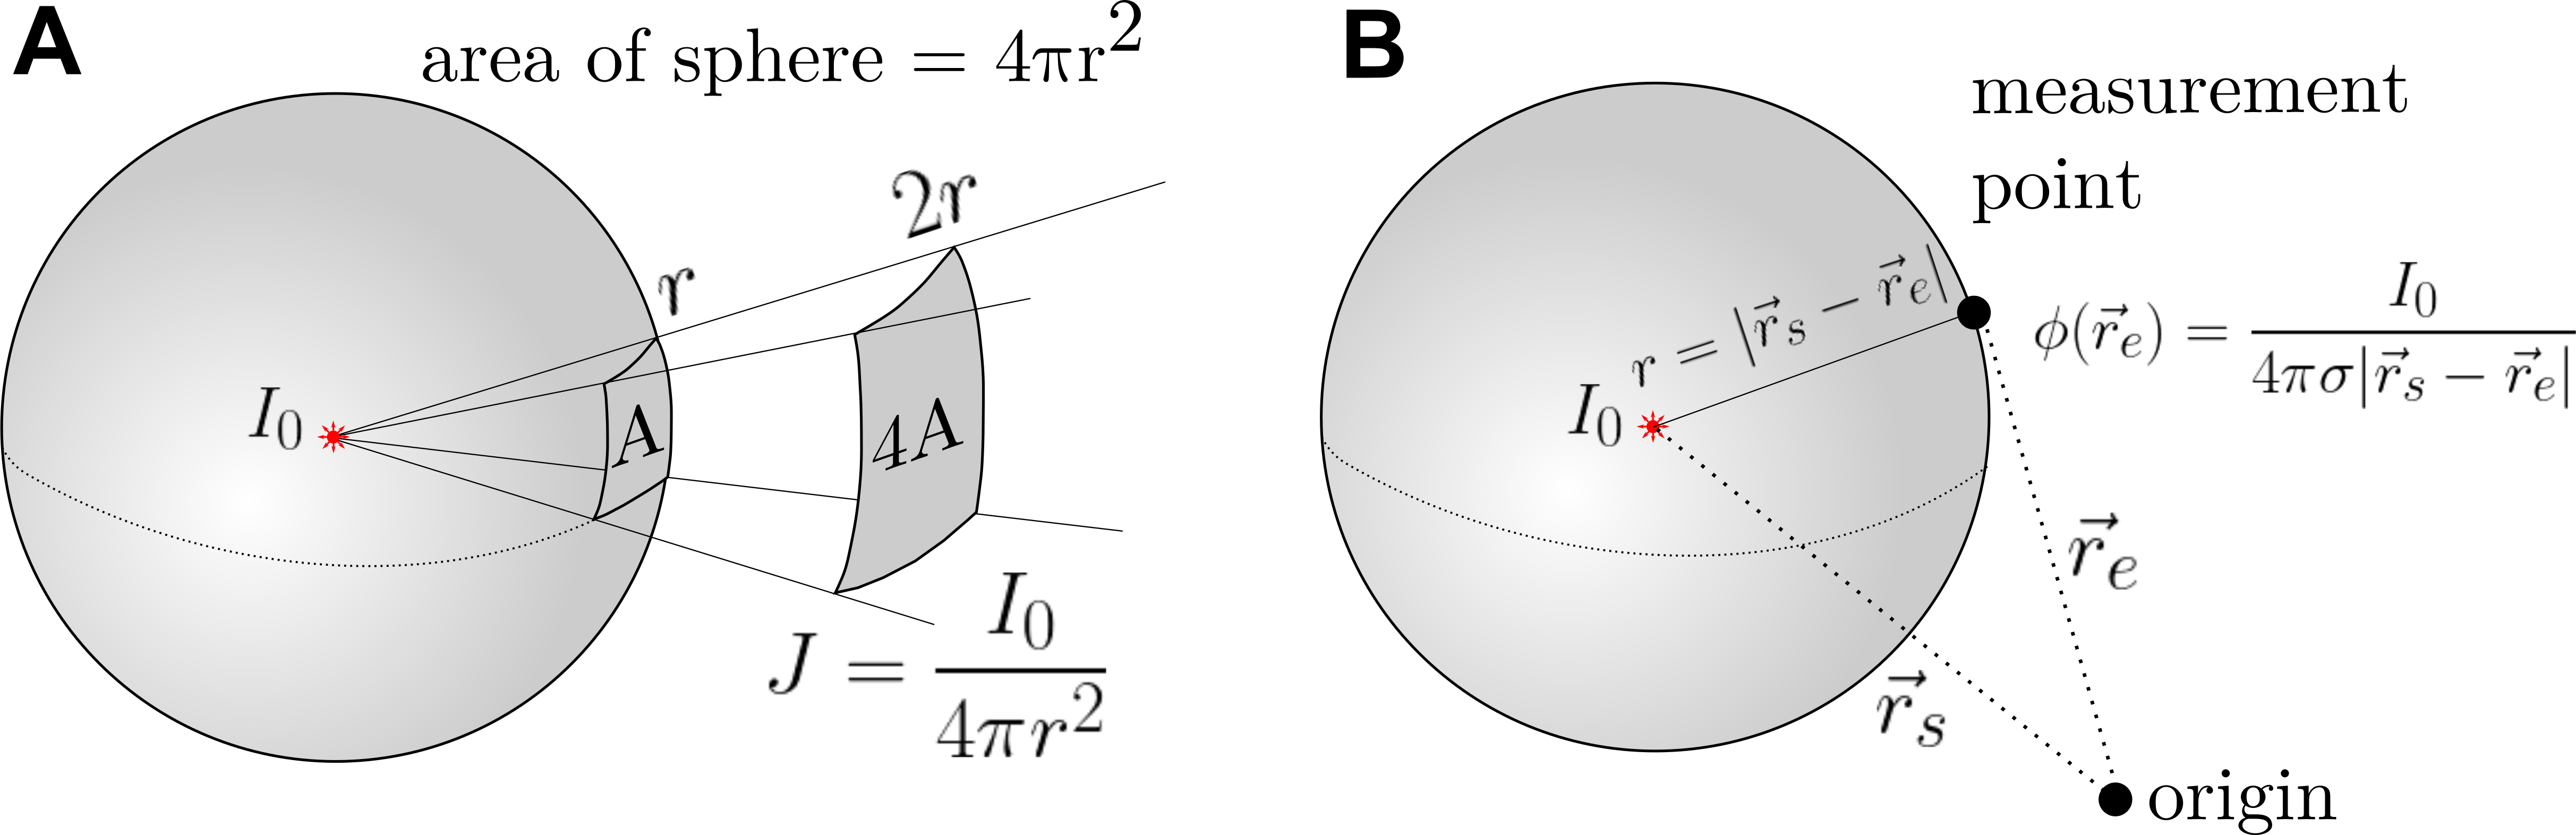
\includegraphics[width=0.8\textwidth]{Figures/VC/EP_from_pointsource_illustration.png}
\end{center}
\caption{\textbf{Extracellular potential from single neuronal point source current.} 
\ghnote{Praktfull, men trenger index $t$ paa $\sigma_t$, og $i_t$ erstatter J.}
}
\label{fig:VC:pointsource}
\end{figure}

Due to the spherical symmetry of this simple case, we know that the current density 
must be radially directed, and that its magnitude must be solely a function of distance $r = |{\bf r}|$ from the source.
In this case, \fref{eq:VC:ohmici} can be written as:

\begin{equation}
i_t({\bf r}) = i_t(r) = -\sigma_t \frac{dV_\mathrm{e}(r)}{dr}.
\end{equation}
\gen{Subscript "t" skal vel ikek vaere i "italics" her?}

Since there can be no charge accumulation anywhere inside the sphere, 
the net current $I_k$ injected into the center of the spherical volume with radius $r$ 
must equal the net current leaving through the surface of the volume. 
The net current leaving the surface can in turn be found by multiplying 
the current density $i_t(r)$ at the surface with the surface area $4\pi r^2$. 
We then get the relationship:
\begin{equation}
I_k = -4\pi \sigma_t r^2  \frac{dV_\mathrm{e}(r)}{dr} \, \iff \, \frac{dV_\mathrm{e}(r)}{dr} = -\frac{I_k}{4\pi \sigma_t r^2 }.
\label{eq:VC:knut}
\end{equation}
\gen{Spandere en egen linje og ligningsnummer paa den siste ligningen?}


To obtain the final solution for $V_\mathrm{e}$, we integrate eq. \ref{eq:VC:knut} from \sntxt{$\infty$ to }$r$:
\begin{equation}
\int_{\infty}^r \frac{dV_\mathrm{e}(r')}{dr'} dr' = \int_{\infty}^r -\frac{I_k}{4\pi \sigma_t r'^2 } dr'.
\label{eq:VC:knut2}
\end{equation}
Since $V_\mathrm{e}({\infty}) = 0$, this leads to the final expression\tvnnote{Skal vaere Ve her og under?}:

\begin{equation}
V({\bf r}) = V(r) = \frac{I_k}{4\pi \sigma_t r},
\label{eq:VC:pointsource}
\end{equation}
where $r$ is the distance from the source.

In the example above, we made things mathematically simple by assuming 
that the current source was placed in the origin ${\bf r} = 0$. \gen{Kanskje ikke boldface siden 0 er en skalar?}
For a point source located in an arbitrary point ${\bf r_k} $ (\fref{fig:VC:pointsource}{\bf B}), 
the corresponding expression for the extracellular potential is:

\begin{equation}
V({\bf r}) = \frac{I_k}{4\pi \sigma_t |{\bf r-r_k}|}.
\label{eq:VC:pointsource2}
\end{equation}

As we stated in the beginning of this chapter, we will assume that the extracellular medium is linear.
This implies that if we have several point-current sources, $I_{1}, I_2, I_3, ... $, 
in locations ${\bf r_1}, {\bf r_2}, {\bf r_3} ... $, 
their contributions add up linearly, and the potential in a point ${\bf r}$ is given by:

\begin{equation}
V({\bf r}) = \frac{I_1}{4\pi  \sigma_t {\bf |r-r_1|}} + \frac{I_2}{4\pi  \sigma_t {\bf |r-r_2|} } + \frac{I_3}{4\pi  \sigma_t {\bf |r-r_3|} } + ... = \sum_k \frac{I_k}{4\pi  \sigma_t {\bf |r-r_k|} }.
\label{eq:VC:pointsources}
\end{equation}

%%%%%%%%%%%%%%%%%%%%%%%%%%%%%%%%
\Fref{eq:VC:pointsources} is referred to as the point-source approximation \cite**{Holt1999}, 
since it approximates the neuron as a set of point current sources, 
i.e., the neuron delivers \sntxt{\sout{to the extracellular space}} a singular current source per neuronal segment \sntxt{to the extracellular space}, 
located in the segment midpoint.


%%%%%%%%%%%%%%%%%%%%%%%%%%%%%%%%
\section{\blue{Line source approximation}}
\label{sec:VC:linesource}
\index{Line source approximation}
Instead of using the point-source approximation, a more sophisticated choice may be 
to assume that the transmembrane current is evenly distributed over the segment axis, 
a choice which is referred to as the \textit{line-source approximation} \cite**{Holt1999,Linden2014}. 
The contribution to the extracellular potential from a current $I_k$ in a segment $k$ 
can be found analytically by integrating \fref{eq:VC:pointsource} over the center-line axis 
of the compartment (see Appendix \ref{app:linesource} or \citeasnoun**{Holt1998}). 
For a segment with length $\Delta s_k$, the contribution to the extracellular potential will be:

\begin{equation}
V_\mathrm{e}({\bf r})_k = \frac{I_k}{4\pi \sigma_t} \int \frac{dr_k}{|{\bf r-r_k}|} =
\frac{I_k}{4\pi \sigma_t \Delta s_k} \log \left| \frac{\sqrt{h_k^2+\rho_k^2}-h_k}{\sqrt{\ell_k^2+\rho_k^2}-\ell_k} \right|.
\label{eq:VC:linesource}
\end{equation}

Here $\rho_k$ is the distance perpendicular to the line segment, 
$h_k$ is the longitudinal distance from the end of the segment, 
and $\ell_k = \Delta s_k + h_k$ is the longitudinal distance 
from the start of the segment (\fref{fig:VC:line_source_illustration}). 
\Fref{eq:VC:linesource} and \fref{eq:VC:pointsource} are the equivalent 
expressions where the transmembrane currents in a single neuronal segment 
are treated as a line source and point source, respectively. 
Like for the point-source approximation, the contributions from 
several line-sources add up linearly. 
That is, if we have multiple segments $k$, 
the extracellular potential can be computed as:

\begin{equation}
V_\mathrm{e}({\bf r}) = \sum_k \frac{I_k}{4\pi \sigma_t \Delta s_k} \log \left| \frac{\sqrt{h_k^2+\rho_k^2}-h_k}{\sqrt{\ell_k^2+\rho_k^2}-\ell_k} \right|.
\label{eq:VC:linesources}
\end{equation}

\begin{figure}[!ht]
\begin{center}
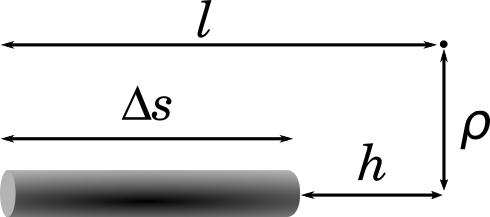
\includegraphics[width=0.5\textwidth]{Figures/VC/line_source_illustration.png}
\end{center}
\caption[]{\textbf{Line-source approximation.} Definitions of symbols used in the line-source approximation. }
\label{fig:VC:line_source_illustration}
\end{figure}

The line-source approximation can be expected to give a better prediction of $V_\mathrm{e}$ 
than the point-source approximation at points in space that are very near neuronal membranes, 
especially when it comes to predicting rapid fluctuations in $V_\mathrm{e}$, 
such as spikes, i.e., extracellular signatures of action potentials \cite**{Holt1999}. 
At points further away from membranes, the two approaches give converging predictions, 
see Fig.~\ref{fig:VC:point_vs_linesource}.

\begin{figure}[!ht]
\begin{center}
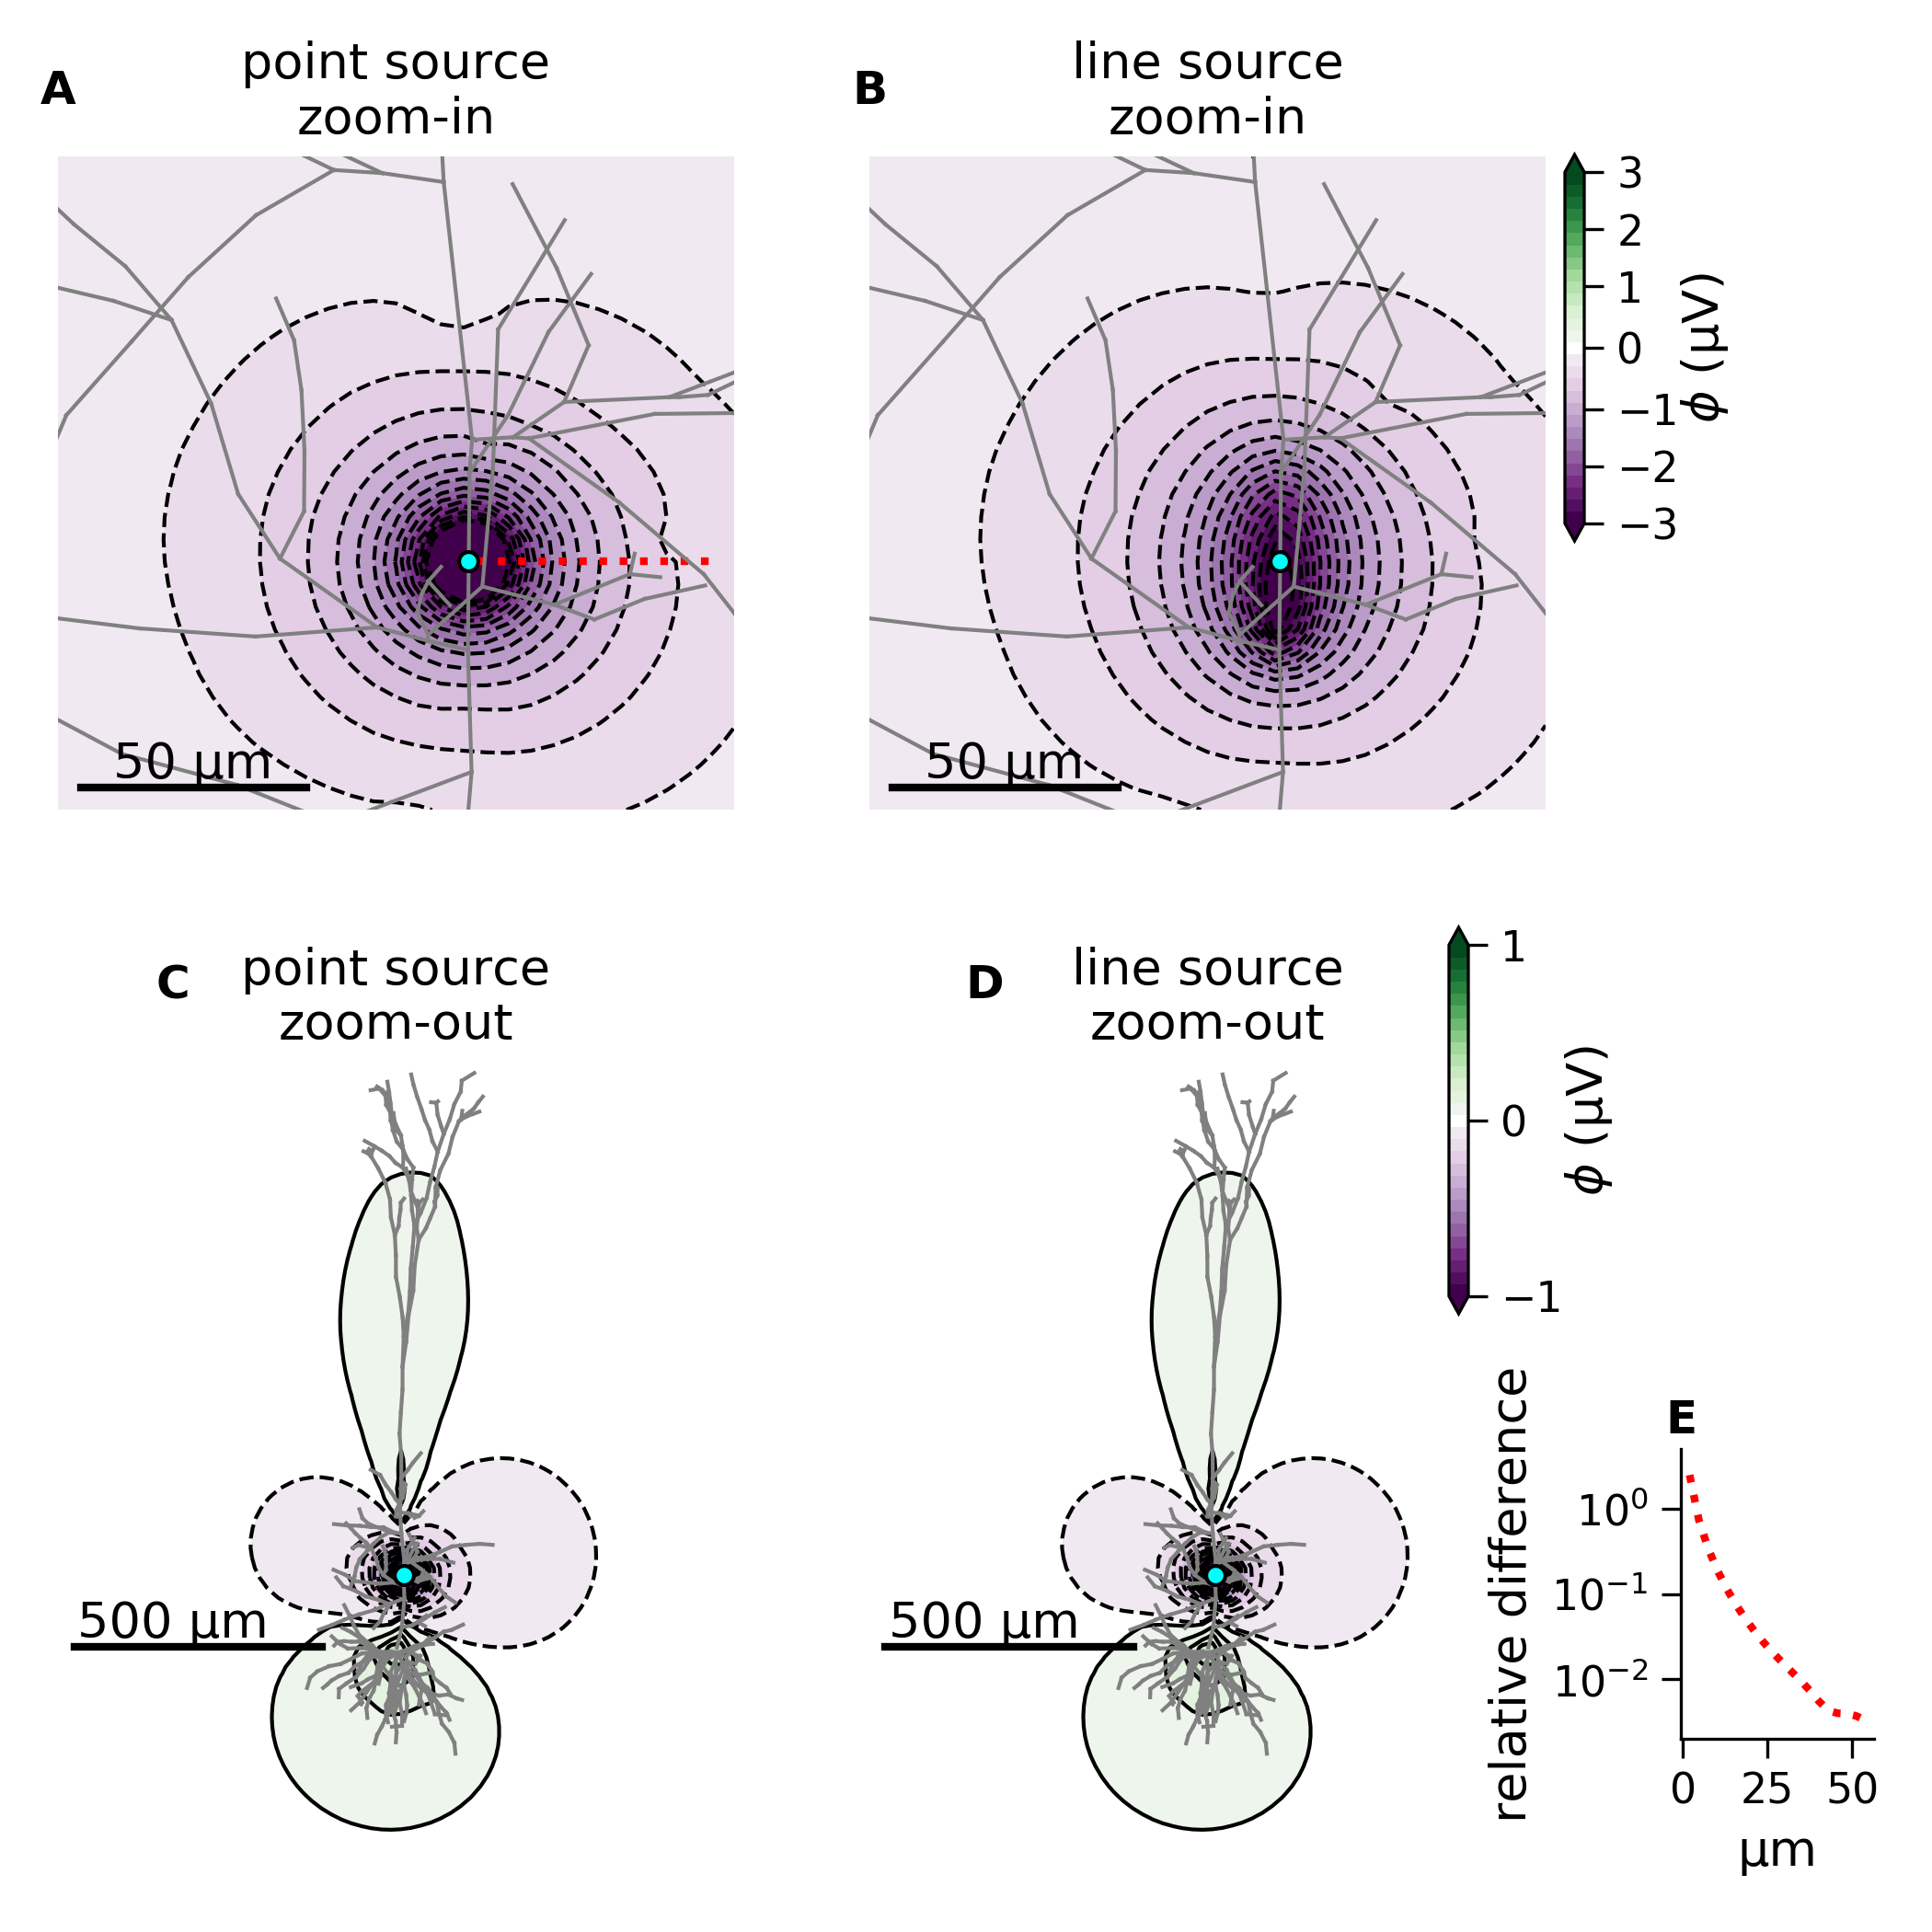
\includegraphics[width=0.7\textwidth]{Figures/VC/fig_point_versus_linesource.png}
\end{center}
\caption[]{\textbf{Point- versus line-source approximation.}
Extracellular potential at a snapshot in time following a single excitatory synaptic input (location marked by cyan dot) to a rat cortical layer 5 pyramidal neuron \cite**{Hay2011}.
The extracellular potential is shown for the time step corresponding to 
the maximum observed absolute value for the extracellular potential, 
and it is calculated from the same neural simulation, at the same time with 
either the point-source approximation ({\bf A}) or the line-source approximation ({\bf B}). 
Very close to neural current sources, the two approaches
give substantially different results, but at slightly larger differences, 
the results from the two approaches converge ({\bf C} versus {\bf D}). 
This is also illustrated in panel {\bf E}, which shows the relative difference 
between the results from the two approaches with increasing distance from the location 
of the synaptic input (red dashed line in panel {\bf A}). 
The relative difference was less than 10\% for distances greater than $\sim$13~\si{\micro\metre}, 
and less than 1\% for distances greater than $\sim$35~\si{\micro\metre}.
}
\label{fig:VC:point_vs_linesource}
\end{figure}


%%%%%%%%%%%%%%%%%%%%%%%%%%%%%%%%
\section{\blue{Current-source-density description}}
\label{sec:VC:CSD}
\index{Current source density}
%%%%%%%%%%%%%%%%%%%%%%%%%%%%%%%%
\gen{Maa vel vaere en bindestrek for mye i overskirften? :-)} 
Instead of representing neural output as a set of point- or line sources, 
we can express it more generally in terms of a spatially continuous density 
of current sources (\fref{fig:VC:CSD}B), $C({\bf r})$, 
which we call the \textit{current source density}\index{Current source density} (CSD), 
with units \si{A/m^3}. 
The extracellular potential evoked by such a distribution can be computed 
from the general continuity equation:
\begin{equation}
\nabla \cdot {\bf i_\mathrm{t}}({\bf r}) = - C({\bf r}).
\label{eq:VC:CSD1}
\end{equation}
What \fref{eq:VC:CSD1} tells us, is that if a neuron outputs a current into a (infinitesimal) 
volume of space (the $C$ term), an equally large current leaves that volume as an 
extracellular current (the $\nabla \cdot {\bf i_t}$ term).

\begin{figure}[!ht]
\begin{center}
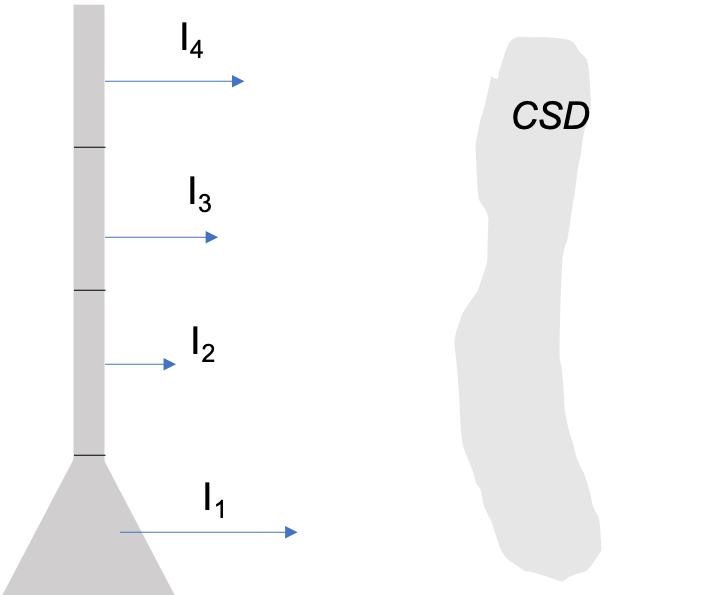
\includegraphics[width=0.5\textwidth]{Figures/VC/CSD.png}
\end{center}
\caption{\textbf{Neuronal current sources.}  
{\bf (A)} When simulated using a numerical scheme, the transmembrane currents 
are known at a discrete set of neuronal segments, i.e., as a set of point sources.  
{\bf (B)} As a mathematical generality, we can describe the transmembrane currents 
as a current source density (CSD) distribution, $C({\bf r},t)$. 
We note the sum of current entering/leaving a neuron is always zero, 
so that in {\bf (A)}, we must have that $I_1 + I_2 + I_3 + I_4 + I_5= 0$, 
and in {\bf (B)} we have that the spatial integral over $C({\bf r},t)$ 
must be zero at all times.
}
\label{fig:VC:CSD}
\end{figure}

If we (as we do throughout the current chapter) assume purely Ohmic extracellular current densities (${\bf i}_\mathrm{t}$) 
and constant, isotropic conductivity ($\sigma_\mathrm{t}$), eq. \fref{eq:VC:CSD1} reduces to a direct relationship 
between the laplacian (double spatial derivative) of the extracellular potential and the transmembrane current sources: 

\begin{equation}
\sigma_\text{t} \nabla^2{V_\mathrm{e}} = -C.
\label{eq:VC:CSD3}
\end{equation}
We have seen these last two equations earlier as \fref{eq:Basics:continuity1} and \fref{eq:Basics:continuity3}. 

If we know the distribution of neuronal current sources, 
we can integrate \fref{eq:VC:CSD3} to predict $V_\mathrm{e}$. 
Since it is a linear differential equation, we can solve it by first finding its Green's function, 
i.e., the solution to an impulse response $C({\bf r}) = I_1 \delta^3({\bf r}-{\bf r}_1)$, 
where $\delta^3({\bf r})$ is the Dirac delta function in three dimensions, 
and $I_1$ represents a singular current source at location ${\bf r}_1$. 
The general solution can then be expressed as a convolution over such Green's functions. 

Thus, we first seek the solution to:
\begin{equation}
\nabla^2 V({\bf r}) = - \frac{I' \delta^3({\bf r-r'})}{\sigma_t}.
\label{eq:VC:CSD5}
\end{equation}

Note that this singular current source is equivalent to the point source that we considered earlier, 
meaning that the solution to this problem is the one that we already found in \fref{eq:VC:pointsource2}. 
Nevertheless, we here provide an alternative (more generally applicable) derivation based on the delta function. 
We start by integrating both sides of \fref{eq:VC:CSD5} over an arbitrary 3D volume $\Omega$ containing the source $I_1$:

\begin{equation}
\iiint_{\Omega} \nabla^2V({\bf r}) \,d\Omega =  - \frac{I'}{\sigma_t} \iiint_\Omega \ \delta^3({\bf r-r'}) \, d\Omega.
\label{eq:VC:marit}
\end{equation}

By the definition of the delta function, the right hand side of \fref{eq:VC:marit} is simply $I_1/\sigma$. 
Using Gauss' theorem, we can convert the volume integral on the left hand side of \fref{eq:VC:marit} 
to an integral over the surface $S$ (enclosing the volume $\Omega$), 
so that \fref{eq:VC:marit} becomes:

\begin{equation}
\oiint_{S} \nabla V({\bf r}) \cdot \, d{\bf S}  = - \frac{I'}{\sigma_t}.
\label{eq:VC:berit1}
\end{equation}
To solve this surface integral, it is convenient to chose the volume that we integrate over 
to be a sphere centered at the source location ${\bf r}_1$, 
and with radius $R = |{\bf r}-{\bf r}_1|$ (\fref{fig:VC:pointsource}{\bf B}). 
Due to the symmetry of problem, we then know that the electric potential 
is the same for all ${\bf r}$ on the spherical surface, so that $V({\bf r}) = V(R)$. 
We also know that its gradient $\nabla V({\bf r}) = d V(R)/dR ~{\bf e}_R$ is constant over the surface, 
and perpendicular to the surface increment $d{\bf S} = dS {~\bf e}_R$. 
If we use this, \fref{eq:VC:berit1} becomes:
\begin{equation}
\oiint_{S} \frac{d V(R)}{dR} d{S}  = - \frac{I_1}{\sigma_t},
\label{eq:VC:berit1ogenhalv}
\end{equation}
which has the solution:
\begin{equation}
4\pi R^2 \frac{d V(R)}{dR} = -\frac{I_1}{\sigma_t}.
\label{eq:VC:berit2}
\end{equation}
If we integrate this from $\infty$ to $R$, and use that $V(\infty) = 0$, we get:
\begin{equation}
V(R) =  \frac{I_1}{4\pi \sigma_t R}.
\label{eq:VC:berit3}
\end{equation}
We may now insert back for $V(R)= V({\bf r})$ and $R = |{\bf r}-{\bf r}_1|$ to obtain the desired Green's function:

\begin{equation}
V({\bf r})= \frac{I_1}{4\pi \sigma_t |{\bf r}-{\bf r}_1|}.
\label{eq:VC:berit4}
\end{equation}
As earlier stated, the solution for a general CSD can be expressed as a convolution over the Green's function, so that:

\begin{equation}
V({\bf r}) = \frac{1}{4\pi \sigma_t}\iiint_{\Omega} \frac{C({\bf r}_s)}{|{\bf r}-{\bf r}_s|} \,d\Omega,
\label{eq:VC:csds}
\end{equation}
where the volume integral runs over all sources with source location denoted ${\bf r}_s$. 
Here, $C$ represents whatever approximation one used for the current sources, 
and \fref{eq:VC:csds} is the continuous counterpart to \fref{eq:VC:pointsources}. 
If we describe the CSD as a sum of point sources, i.e.,  
$C({\bf r}) = \sum_k I_k \delta^3({\bf r} - {\bf r_k})$,  
\fref{eq:VC:csds} reduces to \fref{eq:VC:pointsources}.


\subsection{\blue{Derivation of the current-source density equation}}
\label{sec:VC:C2}
\index{Current source density}
Although the CSD equation (\fref{eq:VC:CSD1}) may seem intuitively reasonable, 
we have so far used it more or less as a postulate. Its theoretical and practical basis
was established in the early works by Charles Nicholson and coworkers
\cite**{Nicholson1971,nicholson1973,nicholson1975,freeman1975},
and a more rigorous derivation was presented later by \citeasnoun**{Gratiy2017}. 
We will not present this derivation in full here, 
but we will walk the interested reader through the main steps. 

The starting point is the conservation law for the total current (density):
\begin{equation}
{\bf \nabla} \cdot {\bf i}_\text{tot} = 0, 
\label{eq:VC:Sergey1}
\end{equation}
which can be defined at any point in space, 
assuming that a continuity description is warranted (cf. \fref{sec:Basics:scale_jump1}).
By "total current density", we simply mean that all current components 
(ohmic, and capacitive when relevant) are included. 

Depending on spatial position, ${\bf i}_\text{tot}$ will vary between being
an intracellular, extracellular or membrane total current density, 
For this reason, \fref{eq:VC:Sergey1} would not be practical to use when describing 
large-scale tissue processes: We would have to map up the detailed structure of brain tissue with high resolution, 
to account for how the very definition of ${\bf i}_\text{tot}$ varies spatially. 

To get around this problem, we seek a version of \fref{eq:VC:Sergey1} 
that is applicable on a larger spatial scale ($\gg 1 \, \si{\cubic\micro\metre}$). 
The diameter of neural dendrites is typically $\sim 1 \,\si{\micro\metre}$, 
which means that a reference volume much greater than this will enclose 
the intracellular spaces of multiple neurites as well as the extracellular space between them. 
The idea is to chose a sufficiently large spatial scale for brain tissue to be homogeneous 
in the sense that any equally sized and arbitrarily placed reference volume will contain roughly 
the same intracellular to extracellular volume fractions (cf. \fref{sec:Basics:scale_jump2}). 
The advantage with such a coarse-grained resolution\index{Coarse-grained} 
is that it introduces a \textit{bi-domain representation}\index{Bi-domain model}, 
where we may think of brain tissue as consisting of two co-existing and interacting domains 
that are both defined continuously over the whole tissue-space, 
rather than within their respective sub-spaces.

To proceed, we define the tissue-coarse grained current $\left<{\bf i}_\text{tot}\right>$ 
as the total current when averaged over the above introduced coarse-grained reference volume. 
Since current conservation must apply also at this larger spatial scale, we have that:

\begin{equation}
{\bf \nabla} \cdot \langle{\bf i}_\text{tot}\rangle = 0.
\label{eq:VC:Sergey2}
\end{equation}

The next trick is to perform the averaging separately over 
the cellular (c) and extracellular (e) domains of the reference volume, so that we can write: 
$\langle{\bf i}_\text{tot}\rangle = \langle{\bf i}_\text{tot}\rangle_\text{c} + \langle{\bf i}_\text{tot}\rangle_\text{e}$, 
where the boundary of the cellular domain(s) run on the external surface of the cellular membranes,
so that $\langle{\bf i}_\text{tot}\rangle_\text{c}$ is the cellular current averaged over the cytoplasm \emph{and} membrane.
With this, \fref{eq:VC:Sergey2} becomes: 

\begin{equation}
{\bf \nabla} \cdot \langle{\bf i}_\text{tot}\rangle_\text{c}  + {\bf \nabla}\cdot \langle{\bf i}_\text{tot}\rangle_\text{e} = 0
\label{eq:VC:Sergey3}
\end{equation}

In \citeasnoun**[Appendix A]{Gratiy2017} it was shown that the divergence of the coarse-grained current density 
over the cellular domain (i.e., the first term on the left in \fref{eq:VC:Sergey3}) 
can be expressed as a sum of transmembrane currents, 
i.e., as a current source density ($C_\mathrm{all}$), like in \fref{eq:VC:CSD1}:

\begin{equation}
{\bf \nabla} \cdot \langle{\bf i}_\text{tot}\rangle_\text{c}  = C_\mathrm{all}.
\label{eq:VC:Sergey4}
\end{equation}
The subfix "all" indicates that the current source density includes all membrane sources present in the tissue, 
and the reason for introducing it will become clear in the net subsection, where we compare 
the theoretically derived CSD equation with the version used in VC theory. 

Further, we define the average current density in the extracellular part of the tissue as, 
\begin{equation}
\langle{\bf i}_\text{tot}\rangle_\text{e} = {\bf i}_\text{e}.
\label{eq:VC:Sergey5}
\end{equation}
where we let it be implicit that ${\bf i}_\text{e}$ is defined on a coarse-grained tissue scale. 
Importantly, ${\bf i}_\text{e}$ denotes the average current running extracellularly through tissue, 
defined as extracellular current per unit \textit{tissue} cross section area 
and not per \textit{extracellular} cross section area 
(although it only runs through the extracellular parts of this cross section area). 


With the definitions in \fref{eq:VC:Sergey4} and \fref{eq:VC:Sergey5}, 
\fref{eq:VC:Sergey3} becomes the CSD equation:
\begin{equation}
\nabla \cdot {\bf i_\mathrm{e}}({\bf r}) = - C_\mathrm{all}({\bf r}).
\label{eq:VC:CSDie}
\end{equation}
The interpretation of this CSD equation is such that if all the sources $C_\mathrm{all}$ are known, 
then ${\bf i}_\text{e}$ is the current density in the (exclusively) extracellular part of tissue. 

\gen{Betyr det at it betyr noe annet her enn tidligere i kapitlet?}
\ghnote{Ja, du hadde et poeng der. Naa heter den $i_e$ og jeg maatte skrive et nytt delkapittel.}


\subsection{\blue{Tissue currents versus extracellular currents}}
\label{sec:VC:C3}
\index{Current source density}
If we compare \fref{eq:VC:CSDie} to the similar \fref{eq:VC:CSD1} used in VC theory:
\begin{equation}
\nabla \cdot {\bf i_\mathrm{t}}({\bf r}) = - C({\bf r}).
\label{eq:VC:CSDit}
\end{equation}
we see that they differ in that the former contains ${\bf i}_\text{e}$ and $C_\mathrm{all}$, 
where the latter contains ${\bf i}_\text{t}$ and $C$. 

The explanation behind this discrepancy 
is that in the theoretical derivation of \fref{eq:VC:CSDie}, $C_\mathrm{all}$ by definition
includes all current sources present in the tissue. Consequently,
the remaining tissue currents exist exclusively in the extracellular subvolume of tissue,
and were therefore denoted ${\bf i}_\text{e}$.

In contrast, when performing forward modeling using the two-step MC+VC scheme, 
we generally have knowledge only of the sources ($C$) that we ourselves have simulated
and impressed onto the tissue. If we do not want to limit VC studies to scenarios where
$C$ accounts for absolutely all membrane currents present in the tissue, we may instead assume
that some (unknown) fraction of the tissue currents evoked by $C$ will cross other (not simulated) 
cellular membranes, so that (i) they travel partially through intracellular pathways (${\bf i}_\text{t} \neq {\bf i}_\text{e}$), 
and thus (ii) evoke(unknown) current sources additional to those simulated ($C \neq C_\text{all}$).
Hence, $C$ in \fref{eq:VC:CSDit} will generally not include all sources present in the tissue, 
and additional (e.g., ephaptically evoked) sources are somehow accounted for
by ${\bf i}_\text{t}$ not being a purely extracellular current. 

As we have seen, the tissue current is normally assumed to be linear and ohmic, 
${\bf i}_\text{t} = \sigma_\text{t} \nabla V_\text{e}$. Assuming that this is true, 
the effective tissue conductivity, $\sigma_\text{t}$, can be found experimentally 
by measuring gradients in $V\text{e}$ evoked by a controlled current injection into the tissue.
In these measurements no assumptions need to be made as to whether the
current pathways between the stimulus and measurement electrode
are purely extracellular or partially intracellular, although there is strong experimental evidence
that the measured magnitude of $\sigma_\text{t}$ reflects that a fair fraction
of the tissue currents take intracellular pathways \cite**{Okada1994}. 

In conclusion, to use VC theory, we do not have to make any assumption
regarding the pathways taken by the currents evoked by the simulated sources $C$. 
However, when assuming the ohmic relationship ${\bf i}_\text{t} = \sigma_\text{t} \nabla V_\text{e}$, 
we implicitly make the assumption that both the intracellular and extracellular 
components of the tissue currents are linearly dependent on the extracellular
potential gradient $\nabla V_\text{e}$.

\ghnote{Og hva skal man si om det? Det er sikkert ok, men laater knappest som noen selvfoelge.}

%\begin{ennumerate}
%\item The tissue currents do not cross any membranes. In this case, they will (i)
%stay confined to the extracellular space (${\bf i_\mathrm{t}} = {\bf i_\mathrm{e}}$), 
%and (ii) will not generate any sources additional to those simulated ($C = C_\text{all}$).
%\Fref{eq:VC:CSDsome} and \fref{eq:VC:CSDall} then become identical.
%
%\item The tissue currents do cross neural membranes. In this case, they will (i) 
%\emph{not} stay confined to the extracellular space (${\bf i_\mathrm{t}} \neq {\bf i_\mathrm{e}}$), 
%but will (ii) generate (unknown) membrane sources in addition to those simulated ($C \neq C_\text{all}$).
%\end{ennumerate}




%%%%%%%%%%%%%%%%%%%%%%%%%%%%%%%%
\section{\blue{Dipole approximation}}
\label{sec:VC:dipole}
The \textit{dipole approximation}\index{Dipole approximation} is an alternative to \fref{eq:VC:pointsources} 
for predicting the extracellular potential. The approximation is good provided that the 
"measuring point" for $V_\mathrm{e}$ is far away from the source-sink distribution that it originates from, 
like in the case of EEG.

To be more precise, if the distance from the center of the volume containing the current sources 
to the measurement point is larger than the maximal distance from volume center to any source \cite**{Jackson1998}, 
we can reformulate \fref{eq:VC:pointsources} by using the the multipole expansion \cite**{Nunez2006}:
\begin{equation}
V_\mathrm{e}({\bf r}) = V_\mathrm{e}(R) = \frac{C_\mathrm{monopole}}{R} + \frac{C_\mathrm{dipole}}{R^2} + \frac{C_\mathrm{quadrupole}}{R^3} + \frac{C_\mathrm{octopole}}{R^4} + ...
\label{eq:VC:multipole}
\end{equation}
where $R = {\bf r} - {\bf r}_c$ is the distance from the center of the source distribution (${\bf r}_c$), 
$C_\mathrm{monopole}$ is the monopolar contribution of the CSD to $V_\mathrm{e}$, 
$C_\mathrm{dipole}$ is the dipolar contribution from the CSD to $V_\mathrm{e}$, 
and so on. The derivation of this expression can be found in Appendix \ref{app:dipoleappendix}.

As we explained in \fref{sec:Neuron:membranecurrents}, 
the net sum of currents over a neuronal membrane is always zero \gex{($C_\mathrm{monopole}=0$)} 
meaning that the monopolar contribution, i.e., first term in \fref{eq:VC:multipole}, vanishes. 
Furthermore, the quadrupole, octopole and higher-order contributions to $V_\mathrm{e}$ 
decay rapidly with distance $R$. Provided that we are sufficiently far away from the source distribution, 
$V_\mathrm{e}$ can therefore be well approximated by the dipole contribution alone:

\begin{equation}\label{eq:VC:CDA}
V_\mathrm{e}({\bf r}) \approx \frac{1}{4 \pi \sigma_t} \frac{|{\bf p}| \cos \theta}{|{\bf r} - {\bf r}_c|^2},
\end{equation}
where we have expressed $C_\mathrm{dipole}$ in terms of the current dipole moment ($\mathbf{p}$) 
and the angle ($\theta$) between the current dipole moment and the distance vector 
($\mathbf{R} = {\bf r} - {\bf r}_c$), as explained in Appendix \ref{app:dipoleappendix}.

The current dipole moment is a function of the sum of all the transmembrane currents in a neuron \cite**{Pettersen2008,Pettersen2014,Nunez2006,Naess2020}:
\begin{equation}
\mathbf{p} = \sum_{k=1}^N I_k \mathbf{r}_k.
\label{eq:VC:dipole}
\end{equation}
For example, if we have a simple two-compartmental (and purely dipolar) neuron with a current sink $-I$ 
at location $\mathbf{r}_1$ and a current source $I$ at location $\mathbf{r}_2$, 
the current dipole moment can be formulated as 
$\mathbf{p} = -I\mathbf{r}_1 + I\mathbf{r}_2 = I(\mathbf{r}_2 - \mathbf{r}_1) = I\mathbf{d}$. 
Here $\mathbf{d}$ is the distance vector between the current sink and the current source, 
giving the length $d$ and direction of the current dipole.

As we mentioned above, 
the current dipole approximation is only applicable when we are at some distance away from the source distribution. 
As a rule of thumb, the approximation is expected to be good when $R$ is three to four times greater than the dipole length: 
$R > 3d$ or $R > 4d$ \cite**{Nunez2006}. \tvnnote{Her hadde det kanskje passet med en figur?}
It has been found to work well for predicting the extracranial EEG signal, 
but less well for intracranial electrocorticography (ECoG) \cite**{Naess2020}.
\gen{Har vi kontroll paa denne "rule of thumb"?}


%\section{\blue{\ghtxt{Modeling \sout{recording electrodes} }recorded potentials}}
\section{\blue{\ghtxt{Modeling recorded potentials} \gex{Modeling recroding electrodes?}}}
\label{sec:VC:electrodes}
\index{Electrode model}
\tvnnote{Paa sikt vil jeg gjerne spoerre noen elektrode-folk vi kjenner om aa kontroll-lese denne seksjonen, for eksempel Martinsen, Nelson, Frey eller Obien.}
%\gen{Kanskje det kunne vaere en ide aa ogsaa beskrive methods-of-imaging og modellering i MEAs her?
%Hadde foerst tenkt aa ta det med i Spikes-kapitlet. Men den gjelder jo like mye for LFP og har blitt brukt av oss i denne
%sammenheng i flere prosjekter med Ness eller Pettersen som foersteforfatter.}
%\tvnnote{Jeg tenker dette passer best i naavaerende 5.3, "Non-homogeneous extracellular medium"?}
Above, we demonstrated how we can use VC theory to predict the extracellular potential ($V_\mathrm{e}$) 
evoked by neural activity. However, in experiments, $V_\mathrm{e}$ must be measured using some kind of electrode, 
and the measurement equipment can in principle affect what is being measured in several ways, 
depending both on electrode properties and features of $V_\mathrm{e}$. 
Below, we present a short review of different approaches to model such effects. 

Recording electrodes essentially consist of an electrode surface in direct contact with neural tissue, 
\gen{Boer kanskje spesifisere at vi ikke snakker om liquid electrodes?}
connected with a wire to an amplifier that measures the potential relative to a reference electrode \cite**{Martinsen2008}, 
see \fref{fig:VC:elec_circuit}{\bf A}. To accurately measure the potential at the electrode surface, 
the measurement electrodes themselves must have a very low resistance 
so that no potential drop occurs from the measurement site to the amplifier. 
The electrodes are therefore typically made of a highly conductive metal like silver or platinum, 
and the potential directly on the inside of the electrode surface is in practice homogeneous. 
In contrast, the amplifier must have a very high impedance \ghtxt{(frequency dependent resistance)}, 
so that a negligible amount of current will cross the tissue-electrode interface, 
as this can cause electrode polarization effects\index{Electrode polarization} \cite**{Schwan1992,Martinsen2008,Moulin2008,Ishai2013}. 
The homogeneous potential inside the recording electrode ideally corresponds to a spatial average 
of the potential across the outer surface of the electrode \cite**{Nelson2008,Nelson2010,Ness2015,Vermaas2020b}.

\begin{figure}[!ht]
\begin{center}
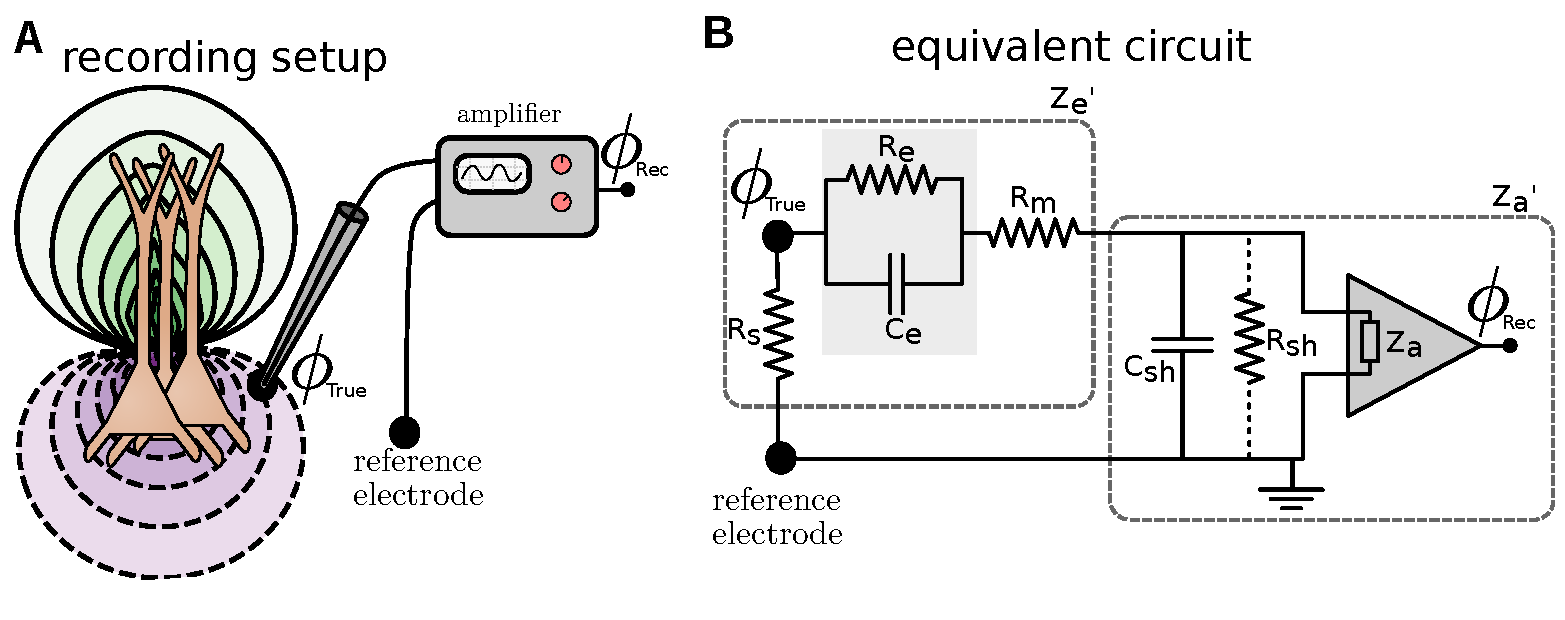
\includegraphics[width=1\textwidth]{Figures/VC/rec_elec_expanded_equivalent_circuit.pdf}
\end{center}
\caption[]{\textbf{Illustration of recording setup and equivalent circuit}
{\bf A}: The extracellular potential is measured between a recording electrode and reference electrode.
{\bf B}: An simple example of an equivalent circuit describing the recording setup, see main text and
\citeasnoun**{Robinson1968}, \citeasnoun**{Nelson2008}, \citeasnoun**{Obien2015}, and \citeasnoun**{Viswam2019}.
}
\label{fig:VC:elec_circuit}
\end{figure}

\ghtxt{
For the sake of examining electrode effects, let us consider a specific recording location, and define for
this location:
\begin{itemize}
\item $V_\mathrm{Phys}$: The "physiological" potential, defined as the $V_\mathrm{e}$ that we \textit{would have} at this location in the absence of any measurement equipment. This is the $V_\mathrm{e}$ that we simulate with VC theory.

\item $V_\mathrm{True}$: The "true" potential, which can differ from $V_\mathrm{Phys}$ if it is affected by the electrode. 

\item $V_\mathrm{Rec}$: The recorded potential, reported by the electrode amplifier system to the experimentalist. 
\end{itemize}
}

\ghtxt{\sout{An "ideal" electrode\index{ideal electrode} is the hypothetical case where the measured potential 
reported by the amplifier is identical to the "true" extracellular potential at the tip of the recording electrode 
(with the extracellular potential unaffected by the electrode itself). 
In reality there are however several different complicating factors which can cause the 
measured potential to differ from the "true" potential Robinson1968,Martinsen2008,Nelson2008}}

\ghtxt{
With an an "ideal" electrode\index{ideal electrode}, $V_\mathrm{Rec}$ would be identical to $V_\mathrm{True}$ 
at the tip of the recording electrode, and $V_\mathrm{True}$ would be unaffected by the electrode itself, 
and thus identical to $V_\mathrm{Phys}$. 
In reality there are however several different complicating factors that can cause the recorded potential 
to differ from the "physiolological" potential \cite**{Robinson1968,Martinsen2008,Nelson2008}.
}
\ghnote{Er dette bedre? Tenkte at sannheten kan vaere sannheten selv om den er paavirket av en elektrode, og proevde aa skille mellom true og physiological.}
\gen{Kan kanskje ogsaa snakke om "ideal point electrode" hvor $V_\mathrm{Rec}$ er lik $V_\mathrm{Phys}$?
Det er jo dette vi stort sett antar.}


%We have demonstrated how we can use VC theory to make predictions about the extracellular potentials at any point in space following some neural activity. However, in experiments these extracellular potentials must be measured through some kind of measurement electrode. The presence of such a measurement electrode might itself affect the measured potentials in several different ways, depending on both the electrode and the extracellular potential that is being measured. 

%\ghtxt{\sout{To understand and/or model such effects it is convenient to represent the recording set-up as an equivalent circuit diagram \cite**{Geddes1997}, see \fref{fig:VC:elec_circuit}{\bf B} for an example inspired by \citeasnoun**{Robinson1968}, \citeasnoun**{Nelson2008}, \citeasnoun**{Obien2015}, and \citeasnoun**{Viswam2019}. Here $V_{\rm e,True}$ is the "true" extracellular potential at some location in the brain, caused by some neural activity, and $V_{\rm Rec}$ is the potential reported by the amplifier. $R_s$ is the resistance of the extracellular medium from the measurement point to the reference electrode. The surface of the electrode, that is, the electrode-electrolyte interface, is often modelled as a resistance, $R_e$, and a capacitance, $C_e$, in parallel (gray shaded area in \fref{fig:VC:elec_circuit}{\bf B}) 
%\cite**{Martinsen2008,Nelson2008,CamunasMesa2013,Viswam2019}. Importantly, the values of both $R_e$ and $C_e$ are typically expected to be highly frequency dependent \cite**{Martinsen2008,Nelson2008,Viswam2019}, and are often considered to be approximately proportional to $1/\sqrt{f}$ \cite**{Robinson1968}, where $f$ is the frequency (implications of this frequency dependence is discussed below).
%The wire from the electrode-electrolyte interface to the amplifier has resistance $R_m$, typically assumed to be negligible.
%$C_{sh}$ and $R_{sh}$ represents all the shunt capacitance and resistance to ground that occurs between the electrode surface and the amplifier, through wires, connections etc., where often $R_{sh}$ is assumed to be negligible.
%Finally, $Z_a$ is the amplifier input impedance.}}

When modeling electrode effects it is convenient to represent the recording set-up as an equivalent circuit diagram \cite**{Geddes1997}. 
An example is shown in \fref{fig:VC:elec_circuit}{\bf B}, where the surface of the electrode 
(the electrode-electrolyte interface), is represented as a resistance, $R_\mathrm{e}$, 
and a capacitance, $C_\mathrm{e}$, in parallel (gray shaded area) \cite**{Martinsen2008,Nelson2008,CamunasMesa2013,Viswam2019}. 
In the figure, $R_\mathrm{s}$ denotes the resistance of the extracellular medium 
from the measurement point to the reference electrode, 
$V_\mathrm{True}$ is the "true" extracellular potential difference between the measurement point and reference electrode, 
while $V_\mathrm{Rec}$ is the potential reported by the amplifier. 
Importantly, the values of both $R_\mathrm{e}$ and $C_\mathrm{e}$ are typically 
expected to be highly frequency dependent \cite**{Martinsen2008,Nelson2008,Viswam2019}, 
and are often considered to be approximately proportional to $1/\sqrt{f}$ \cite**{Robinson1968}, 
where $f$ is the frequency of the recorded signal (implications of this frequency dependence is discussed below). 
The resistance of wire from the electrode-electrolyte interface to the amplifier is denoted $R_\mathrm{m}$, 
and is typically assumed to be negligible. 
$C_\mathrm{sh}$ and $R_\mathrm{sh}$ represent all the shunt capacitance and resistance to ground 
that occur between the electrode surface and the amplifier, through wires, connections etc., 
where often $R_\mathrm{sh}$ is assumed to be negligible. Finally, $Z_a$ is the amplifier input impedance.

Two important concepts in \fref{fig:VC:elec_circuit}{\bf B} are the effective electrode impedance, $Z_e'$, 
and the effective amplifier input impedance, $Z_a'$. The former is the combined impedance of the 
extracellular medium ($R_s$), the electrode-electrolyte interface ($R_e$, $C_e$) and the metal wire ($R_m$), 
while the latter is the total impedance to ground from after the metal wire, 
and includes the shunt currents and the amplifier itself. 
For the recorded potential, $V_{\rm Rec}$ to be as similar as possible to the true potential, $V_{\rm True}$,  
it is vital that $Z_a' \gg Z_e'$. 
If this is not fulfilled, the recorded potential will have frequency-dependent phase- and amplitude distortions \cite**{Nelson2008,Nelson2010,Obien2015,Viswam2019}.
Importantly, the effective electrode impedance, $Z_e'$, increases strongly for low frequencies 
and is typically much more frequency dependent than the effective amplifier input impedance, 
$Z_a'$ \cite**{Nelson2008}. 
This means that some given recording equipment might be able to measure \ghtxt{rapidly varying signals, such as}
extracellular spikes, with negligible distortion, while at the same time substantial 
phase and amplitude distortions might be present in \ghtxt{slower signals, such as local field potentials,} 
\ghtxt{\sout{LFP signals}} measured with the same equipment \cite**{Nelson2008,Nelson2010,Viswam2019}.

Note that \tvntxt{\sout{metallic recording electrodes are typically} the measurement equipment typically used in neuroscience is} unable to measure static (DC) potentials, 
or capture changes slower than $\sim$ 0.1 Hz.
Such DC potentials can be present in neural tissue, and can often arise in simulated 
extracellular potentials from cell models with active conductances, for example because of the 
$I_{\rm h}$-current \cite**{Ness2016}. In such cases, the simulated baseline (or mean) 
extracellular potential is typically subtracted from the extracellular potentials to effectively 
remove the unobservable DC-potential.

\gen{Hvor har vi dette tallet fra?}
\ehnote{jeg er ogsaa overrasket over at metallelektroder ikke kan maale konstante potensialforskjeller i en loesning (i all den tid det finnes frie ioner i loesningen)?}
\tvnnote{Jeg vet ikke om noen laerebok referanse, men det var det som ble oppgitt som nedre grense baade av Dirk og Anna (altsaa alle tilfeller jeg har vaert borti eksperimentell data), se Miceli-artikkelen, Uhlivora-artikkelen, og ogsaa Einevoll et al., 2007. Fra en av Anna's nyere artikler fant jeg frem til dokumentasjonen paa amplifieren de har brukt, og der staar det "Lower cutoff frequency configurable from 0.1 Hz to 500 Hz", men jeg vet ikke helt om forklaringen jeg har gitt over er helt riktig.}
\ehnote{Det er vel da mer en begrensning med sampling apparat enn selve elektrodemaalingen. Si du sampler mange kanaler med int16 presisjon - det blir da et problem hvis DC-verdiene fluktuerer mye mer enn selve signalet (e.g., LFP).}
\gen{Slik jeg forstod det da jeg snakket med Ulbert om saken i urtiden er det alltid et DC "kontaktpotensial" mellom metallkontakter og elektrolytter. Dette er i praksis ukjent og vil variere fra kontakt til kontakt, f.eks., i en MEA. Ulbert sa at DC potensialer derfor kun kunne maales med liquid elektroder.}

%\begin{figure}[!ht]
%\begin{center}
%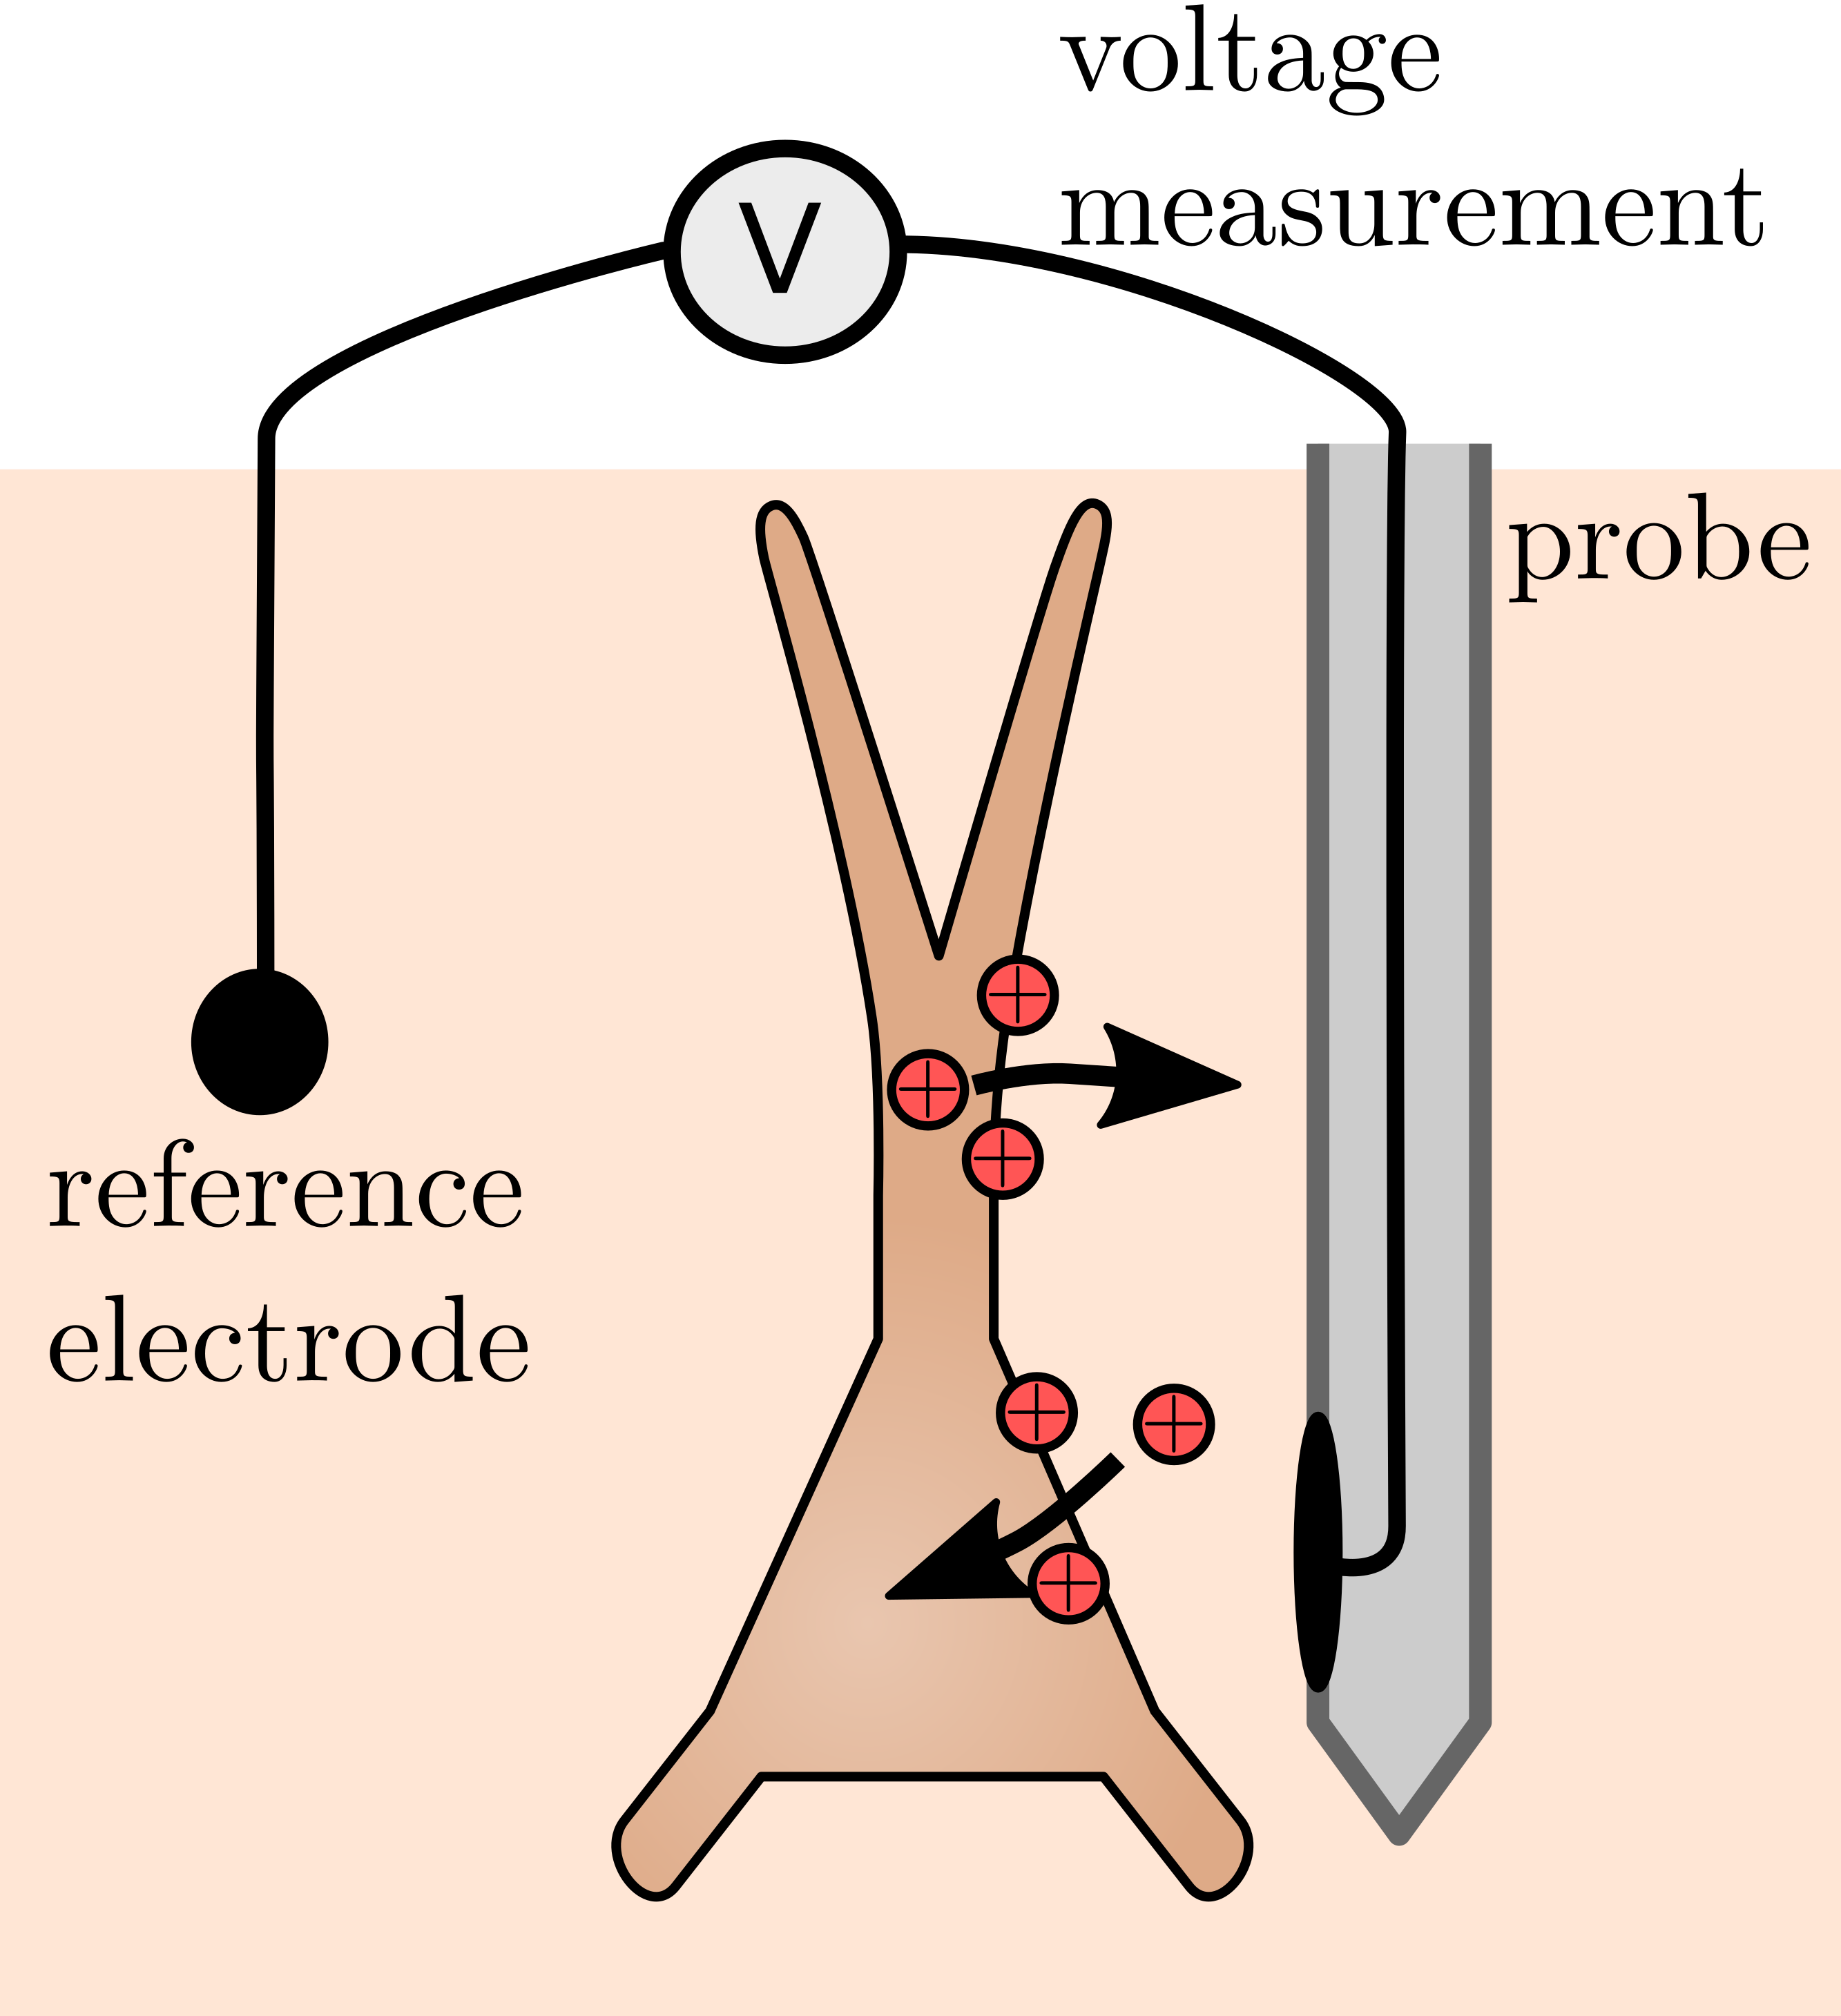
\includegraphics[width=0.4\textwidth]{Figures/VC/rec_elec_circuit.png}
%\end{center}
%\caption[]{\textbf{Illustration of recording circuit}
%Electric potential is measured between recording electrode and reference electrode, and represents the energy required to move a positive test charge from the reference electrode and to the measurement electrode. If, say, positive ions are leaving the extracellular medium (and entering a cell) in the vicinity of the recording electrode, then the energy needed to move a positive charge to the measurement electrode is negative, that is, one can gain energy by moving the charge there.  \ghnote{Litt usikker paa energi-betraktningene her. Dvs. ikke paa om de er riktige, men om de hjeper leseren...} \tvnnote{Ja, enig. Men jeg foeler det hadde vaert fint aa forklare et sted hvorfor for eksempel negatv transmembran stoem gir negativt maalt potensial. Kunne denne figuren (eller noe lignende) vaert med i for eksempel seksjon 2.3?}
%}
%\label{VC:fig:elec_circuit}
%\end{figure}

Apart from the issues discussed above \ghnote{Hvilke issues? Alle? De som angaar DC-potensialet? Eller mener vi "despite the issues?"}\tvnnote{Jeg tenkte paa DC-potensialet. Min forstaaelse av dette er at siden Ze er veldig frekvens-avhengig, blir ikke Za' mye stoerre enn Ze' naar f er liten, men jeg vet ikke om dette er riktig tolkning.}, it has been convincingly argued that, provided that the proper recording equipment is used (so that $Z_a' \gg Z_e'$), 
electrode impedance or other electrode properties should not substantially distort recorded potentials 
\ghtxt{i.e., we can assume that  $V_\mathrm{True} \approx V_\mathrm{Phys}$} \tvnnote{Ha med VRec?} \cite**{Martinsen2008,Moulin2008,Nelson2008,Nelson2010}.
Note that this only applies to recording electrodes, and that substantially more complex 
electrode models might be needed to accurately represent current stimulation electrodes 
because of electrode polarization, see \fref{sec:EPI}.

\ghnote{Hang ikke helt med. I avsn. over sto det "electrode properties should not distort recorded potentials. Under staar det electrode properties can still affect the recorded potential. Hva er forskjellen? Tipper at du foerst mente at elektroden er slik at $V_\mathrm{True} = V_\mathrm{Phys}$, men i neste tilfelle at det ikke noedvendigvis er slik at $V_\mathrm{Rec} \neq V_\mathrm{True}$. Har laget en versjon basert paa den forstaaelsen.}

Under the assumption that the proper recording equipment is used \cite**{Nelson2008,Nelson2010}, 
electrode properties \ghtxt{\sout{can still affect the}} \ghtxt{will nevertheless affect the relationship between the true potential and the} recorded potential \ghtxt{so that $V_\mathrm{Rec} \neq V_\mathrm{True}$}. For example, since the (homogeneous) potential directly on the inside of the electrode surface corresponds to a spatial average of the potential on the outside, the area of the electrode surface will affect how large a region the extracellular potential is averaged over. In practice, this means for example that extracellular \ghtxt{\sout{action potentials}spikes} (which are very spatially confined) will be less prominent on electrodes with diameters larger than $\sim$30~\si{\micro\metre} \cite**{Moffitt2005,Moulin2008,Viswam2019}, see \fref{sec:Spikes:electrode_size}. \ghnote{Kan dette skrivers klarere? Less prominent when larger than 30 mum - less than what, hvorfor 30? Antar det kan skrives generelt: Less prominent the larger the diameter. Er dette rett: Difficult to detect when larger than 30 mum?}

%if the extracellular potential changes across the outer surface of the recording electrode, this can introduce a spatial filtering effect on the measured potentials.
%\gen{Her maa vi vaere presise. Potensialet paa selve elektroden vil vaere det samme, det som vil variere er hva potensialet ville vaert paa denne "virtuelle" flaten hvis det ikke hadde vaert en metallisk elektrode der.}
%In practice, this means for example that extracellular action potentials (which are very spatially confined) will be less prominent on electrodes with diameters larger than $\sim$30~$\mu$m \cite**{Moffitt2005,Moulin2008,Viswam2019}, see Section~\ref{Spikes:sec:elec_size}.


\subsection{\blue{Point-electrode approximation}}
\label{sec:VC:point-electrode}
\index{Point-electrode}

\gen{Burde noe av teksten over vaert i en egen subsection?}

The most straightforward and also most common approach when modeling extracellular recordings is to use the ideal point electrode approximation. This corresponds to ignoring \ghtxt{\sout{any potential effect}possible effects} from recording electrodes or electrode shanks, \ghtxt{assuming that the recorded potential, $V_\mathrm{Rec}$, is identical to the physiological potential, which in turn is identical to $V_\mathrm{e}$ as computed using VC theory.} \ghtxt{\sout{and calculating 
the extracellular potential at single points.}} For relatively small micro-electrodes this has been found to be a reasonable approximation \cite**{Moffitt2005,Moulin2008,Ness2015,Buccino2019}.
\ghnote{Er ikke det rett: Point-electrode approximation = VC-teori uten no knussel?}
\gen{Men i prinsipp kunne man vel ha en daarlig amplifier. Saa det er vel "ideal" point-electrode approximation som tilsvarer knusselfri VC-teori?}

\subsection{\blue{Disc-electrode approximation}}
\label{sec:VC:disc-electrode}
\index{Disc-electrode approximation}
\ghtxt{\sout{In some cases recording electrodes are large enough that the the extracellular potential}
Under some experimental conditions  $V_\mathrm{e}$} varies substantially across the electrode surface, 
either because the electrodes are large (like ECoG electrodes at the cortical surface), 
or because \ghtxt{\sout{the extracellular potential}$V_\mathrm{e}$} varies substantially over small distances 
(like extracellular spikes from axons). 
In such cases, we can use \ghtxt{\sout{the point-electrode approximation}VC-theory}\tvnnote{syntes det er fint aa ha med at dette egentlig bare er en triviell utvidelse av punk-kilde approksimasjonen} to calculate \ghtxt{\sout{the potential}$V_\mathrm{e}$} at \ghtxt{\sout{many}all} points across the electrode surface 
and compute the average potential \ghtxt{as a proxy for $V_\mathrm{Rec}$}, 
an approach referred to as the disc-electrode approximation \cite**{CamunasMesa2013,Linden2014,Hagen2015,Ness2015,Viswam2019}. 
\ghtxt{\sout{This approach takes into account}The disc-electrode approximation accounts for} the physical extent of the electrodes, \ghtxt{\sout{and the disc-electrode approximation can therefore account} and therefore also} for the spatial filtering effects introduced by electrodes that are large compared to the spatial variations of the \ghtxt{\sout{extracellular potential}$V_\mathrm{e}$}. See \fref{sec:Spikes:electrode_size} for an example of this approach applied to calculating extracellular 
spikes recorded with electrodes of different sizes.

However, very close to electrodes the electrodes can themselves affect the close-by extracellular potential, 
since they represent a region of a highly conductive material in contact with the tissue being measured from.
The effect of the presence of highly conductive electrodes can be investigated using the Finite Element Method (FEM) \index{Finite Element Method}. \citeasnoun**{Ness2015} found that the disc-electrode approximation was fairly accurate for estimating measured potentials from a point current source more than $\sim$2 times the electrode radius away from the electrode. The point-electrode approximation was \ghtxt{\sout{also}} found to be fairly accurate for distanced greater than $\sim$4 times the electrode radius away from the electrode, see \fref{fig:VC:FEM_elec}.

\begin{figure}[!ht]
\begin{center}
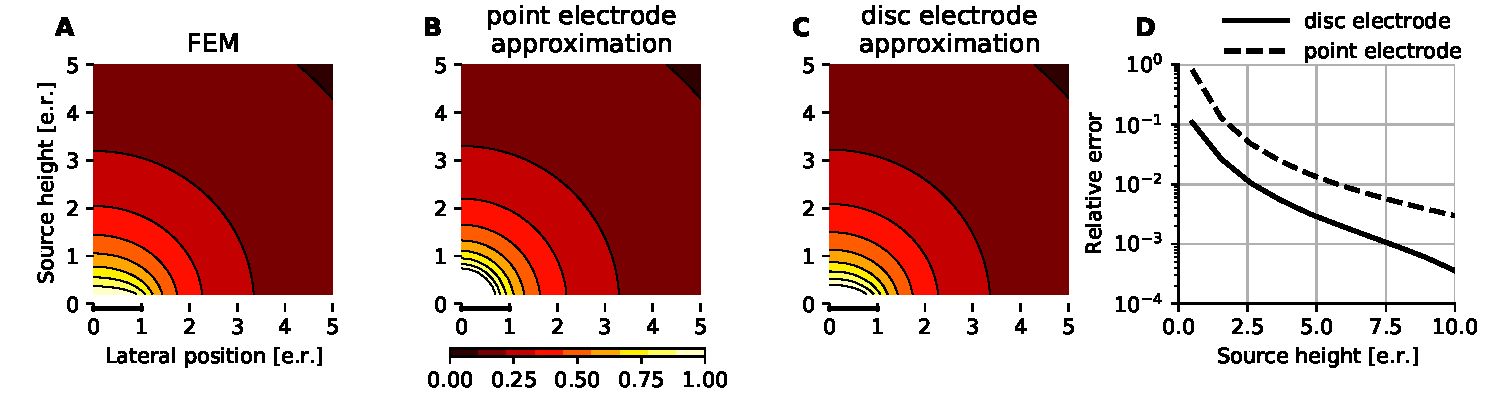
\includegraphics[width=1\textwidth]{Figures/VC/fig_FEM_elec.pdf}
\end{center}
\caption[]{\textbf{Finite Element Method versus the point and disc electrode approximations.}
{\bf A:} The lead-field from an electrode surface at $x$,$y$=0, simulated with the Finite Element Method (FEM). The highly conductive material of the electrode was included in the simulation, as a cylinder protruding out of the bottom of an otherwise homogeneous and isotropic volume conductor. The $x$- and $y$-axes are shown in units of the electrode radius, which in this specific example was 10~\si{\micro\metre}.
{\bf B:} The lead-field from a point current source at the bottom of an homogeneous and isotropic volume conductor, $x$,$y$=0.
{\bf C:} The lead-field from 500 point current source randomly distributed across the electrode surface, centered at $x$,$y$=0. Each current source was scaled by 1/500.
The Method of Images (Sec.~\ref{sec:Sigma:nonhomo}) was used to account for the bottom of the volume for the point- and disc-electrode approximation.
See \citeasnoun**{Ness2015} for full simulation details.
}
\label{fig:VC:FEM_elec}
\end{figure}

In certain cases, like in ECoG \index{ECoG} measurements from the cortical surface, the recording electrodes are both large ($\sim$~2-5~mm diameter) and close to the neuronal sources (the thickness of the human cortex is $\sim$3~mm). In such cases the electrode properties can therefore be expected to have large effect on measured potentials, see for example \citeasnoun**{Vermaas2020b} and \citeasnoun**{Rogers2020}.

\gen{Her maa vi sjekke:} \citeasnoun**{Viswam2019}

\subsection{\blue{Effect of the electrode shanks}}
\label{sec:VC:elec_shafts}
Large multi-contact electrode shanks can be expected to have a substantial effect on close-by extracellular potentials, since they represent large, non-conducting volumes \cite**{Moffitt2005,Lempka2011,Mechler2012,Buccino2019}. It has been demonstrated that such large probes can amplify or dampen recorded potentials from nearby cells by almost a factor of two, depending on whether the cell was in front of or behind the electrode shank \cite**{Moffitt2005,Buccino2019}, while no such effects were found for small microwires \cite**{Buccino2019}. \tvnnote{Can also hurt the brain to push large objects into it, with cell-death, eudema and encapsulation (Moffitt and McIntyre, 2005).}
\gen{Virkelig? Da maa jeg slutte med det .. :-)} 
%%%%%%

\subsection{\blue{Effect of position of reference electrode}}
\label{sec:VC:ref_elec}
\ghnote{En eventuell diskusjon av hvor man plasserer referanseelektrodene kan inngaa her. Kommentarene under er sakset inn fra tidligere diskusjoner i Basics-kapittelet:} 
\tvntxt{When recording extracellular potentials in the brain, we are in principle free to arbitrarily choose the location of the reference electrode. The ideal location for the reference electrode depends on several different factors, but it is commonly placed "far away" from the neural activity that is being measured from so that the measured potential is not dependent on an unknown varying electrical activity around the reference electrode. When modelling extracellular potentials, the reference electrode is typically (and often implicitly) placed at "infinity". } \ghnote{Stemmer egentlig dette? Slik jeg forsto Sharott vil man i motsetning til det dere skriver ofte ha referanseelektroden naer maaleelektroden naar man maaler MUA, for paa den maaten aa filtrere bort effekter fra "nest naermeste nabo". Hva var galt med mitt (mer vage) forslag:} \ghtxt{When we record extracellular potentials in the brain, we can choose to place the reference electrode close or far away from the recording electrode, depending on the kind of signal one wishes to measure \cite**{Sharott2015}.} \ghnote{Kanskje si: Naar man modellerer er den i infinity. Stort sett skal vaere langt unna.} \gen{Kanskje si enda klarere at man oensker at potensialet paa referanseelektroden skal vaere saa konstant som mulig under eksperimentet (eller blir dette sirkulaert?), husker at Anna plasserte referanseelektroden i nakken paa rottene hun gjorde maalinger fra. Kanskje vi kan hoere med eksperimentalistene paa CINPLA hva de gjoer?} \ghnote{Sikkert lurt aa spoerre noen, ja, men saa vidt jeg skjoenner er dette et vanskelig spoersmaal der mange avveininger maa gjoeres.} \ghnote{Poenget er aa plassere den der det er mest praktisk - best mulig signal for det du er ute etter. }
\snnote{Jeg snakket med Malin og de pleier aa gjoere det slik: For LFP-maalinger pleier de aa sette en jordingsskrue paa skallen, ganske langt unna der maaleelektrodene skal settes ned (for aa unngaa aa skade maaleomraadet.) Dette kommer i tillegg til jording av selve systemet. For MUA-maalinger har de i tillegg en referanseelektrode per elektrode, og denne vil vaere plassert i naerheten av maaleelektroden, et sted der raasignalet er mest mulig likt. Istedenfor referanseelektrode kan de evt bruke en median/snitt-verdi for alle kanaler i en hemisfaere, evt innenfor en tetrode.}




\section{\red{Validation of framework}}
\tvnnote{Jeg foeler vi typisk skriver "extracellular potentials can be modelled by well-established VC theory", og sleger paa en sitering til en kilde som vel egentlig bare sier akkurat det samme.
 Jeg har lyst til aa dedikere litt plass til
"validering". Type: Hvilke beviser finnes for at ECP kan modelleres med transmembrane stroemmer fra kabel-ligning kombinert med VC?}

\ghnote{Lykke til!}
\tvnnote{Takk takk :-) Men det at det virker veldig ambisioest og argumentere for at selve hoved-rammeverket vaart, som vi selv har stor tiltro til, i det hele tatt er gyldig, kan jo ogsaa sees paa som et argument for at det er viktig aa gjoere det :-)}

\gex{Absolutt en god ide aa samle argumenter for hvorfor vi tror paa vaart framework. 
Det viktigste argumentet er vel at MC og VC er validert godt hver for seg, men ogsaa 
beregnede spikes og LFPs har stemt rimelig godt med eksperimenter.
Her er starten paa en liste:
\begin{itemize}
\item MC
\begin{itemize}
\item Antagelsen om at MC modellering (kabelligning) fungerer for aa regne ut intracellulaere membranpotensialer er vel rimelig godt bekreftet, going back to Hodgkin og Huxley og aksonet deres
\item Antagelsen om at MC modellering (kabelligning) derved fungerer for aa regne ut transmembrane strommer er vel kanskje ikke sjekket direkte mot eksperimenter(?), men det er er rimelig aa tenke at dette maa fungere ogsaa, gitt at 
MC fungerer for intracellulaere membranpotensialer 
\item ...
\end{itemize}
\item VC
\begin{itemize}
\item VC-antagelsen om relasjonen mellom injisert str{\o}m og maalte potensialer er godt bekreftet for stroemmer injisert med elektroder, fra centimeterskala og vel egentlig ned til 0.1 mm skala \cite{Miceli2017}
\item ....
\end{itemize}
\item MC+VC 
\begin{itemize}
\item Beregnede spikes ligner til dels veldig paa det som sees eksperimentelt, cf. \Fref{fig:Spikes:Henze}. Dette er ogsaa for smaa avstander hvor vel VC antagelsen ikke er testet direkte.
\item Beregnet unitary thalamocortical LFP ligner veldig paa det som sees eksperimentelt \cite{Hagen2017}
\item ...
\end{itemize}
\end{itemize}
}
